% Options for packages loaded elsewhere
\PassOptionsToPackage{unicode}{hyperref}
\PassOptionsToPackage{hyphens}{url}
\PassOptionsToPackage{dvipsnames,svgnames,x11names}{xcolor}
%
\documentclass[
  letterpaper,
  DIV=11,
  numbers=noendperiod]{scrartcl}

\usepackage{amsmath,amssymb}
\usepackage{iftex}
\ifPDFTeX
  \usepackage[T1]{fontenc}
  \usepackage[utf8]{inputenc}
  \usepackage{textcomp} % provide euro and other symbols
\else % if luatex or xetex
  \usepackage{unicode-math}
  \defaultfontfeatures{Scale=MatchLowercase}
  \defaultfontfeatures[\rmfamily]{Ligatures=TeX,Scale=1}
\fi
\usepackage{lmodern}
\ifPDFTeX\else  
    % xetex/luatex font selection
\fi
% Use upquote if available, for straight quotes in verbatim environments
\IfFileExists{upquote.sty}{\usepackage{upquote}}{}
\IfFileExists{microtype.sty}{% use microtype if available
  \usepackage[]{microtype}
  \UseMicrotypeSet[protrusion]{basicmath} % disable protrusion for tt fonts
}{}
\makeatletter
\@ifundefined{KOMAClassName}{% if non-KOMA class
  \IfFileExists{parskip.sty}{%
    \usepackage{parskip}
  }{% else
    \setlength{\parindent}{0pt}
    \setlength{\parskip}{6pt plus 2pt minus 1pt}}
}{% if KOMA class
  \KOMAoptions{parskip=half}}
\makeatother
\usepackage{xcolor}
\setlength{\emergencystretch}{3em} % prevent overfull lines
\setcounter{secnumdepth}{-\maxdimen} % remove section numbering
% Make \paragraph and \subparagraph free-standing
\ifx\paragraph\undefined\else
  \let\oldparagraph\paragraph
  \renewcommand{\paragraph}[1]{\oldparagraph{#1}\mbox{}}
\fi
\ifx\subparagraph\undefined\else
  \let\oldsubparagraph\subparagraph
  \renewcommand{\subparagraph}[1]{\oldsubparagraph{#1}\mbox{}}
\fi


\providecommand{\tightlist}{%
  \setlength{\itemsep}{0pt}\setlength{\parskip}{0pt}}\usepackage{longtable,booktabs,array}
\usepackage{calc} % for calculating minipage widths
% Correct order of tables after \paragraph or \subparagraph
\usepackage{etoolbox}
\makeatletter
\patchcmd\longtable{\par}{\if@noskipsec\mbox{}\fi\par}{}{}
\makeatother
% Allow footnotes in longtable head/foot
\IfFileExists{footnotehyper.sty}{\usepackage{footnotehyper}}{\usepackage{footnote}}
\makesavenoteenv{longtable}
\usepackage{graphicx}
\makeatletter
\def\maxwidth{\ifdim\Gin@nat@width>\linewidth\linewidth\else\Gin@nat@width\fi}
\def\maxheight{\ifdim\Gin@nat@height>\textheight\textheight\else\Gin@nat@height\fi}
\makeatother
% Scale images if necessary, so that they will not overflow the page
% margins by default, and it is still possible to overwrite the defaults
% using explicit options in \includegraphics[width, height, ...]{}
\setkeys{Gin}{width=\maxwidth,height=\maxheight,keepaspectratio}
% Set default figure placement to htbp
\makeatletter
\def\fps@figure{htbp}
\makeatother

\KOMAoption{captions}{tableheading}
\makeatletter
\makeatother
\makeatletter
\makeatother
\makeatletter
\@ifpackageloaded{caption}{}{\usepackage{caption}}
\AtBeginDocument{%
\ifdefined\contentsname
  \renewcommand*\contentsname{Table of contents}
\else
  \newcommand\contentsname{Table of contents}
\fi
\ifdefined\listfigurename
  \renewcommand*\listfigurename{List of Figures}
\else
  \newcommand\listfigurename{List of Figures}
\fi
\ifdefined\listtablename
  \renewcommand*\listtablename{List of Tables}
\else
  \newcommand\listtablename{List of Tables}
\fi
\ifdefined\figurename
  \renewcommand*\figurename{Figure}
\else
  \newcommand\figurename{Figure}
\fi
\ifdefined\tablename
  \renewcommand*\tablename{Table}
\else
  \newcommand\tablename{Table}
\fi
}
\@ifpackageloaded{float}{}{\usepackage{float}}
\floatstyle{ruled}
\@ifundefined{c@chapter}{\newfloat{codelisting}{h}{lop}}{\newfloat{codelisting}{h}{lop}[chapter]}
\floatname{codelisting}{Listing}
\newcommand*\listoflistings{\listof{codelisting}{List of Listings}}
\makeatother
\makeatletter
\@ifpackageloaded{caption}{}{\usepackage{caption}}
\@ifpackageloaded{subcaption}{}{\usepackage{subcaption}}
\makeatother
\makeatletter
\@ifpackageloaded{tcolorbox}{}{\usepackage[skins,breakable]{tcolorbox}}
\makeatother
\makeatletter
\@ifundefined{shadecolor}{\definecolor{shadecolor}{rgb}{.97, .97, .97}}
\makeatother
\makeatletter
\makeatother
\makeatletter
\makeatother
\ifLuaTeX
  \usepackage{selnolig}  % disable illegal ligatures
\fi
\IfFileExists{bookmark.sty}{\usepackage{bookmark}}{\usepackage{hyperref}}
\IfFileExists{xurl.sty}{\usepackage{xurl}}{} % add URL line breaks if available
\urlstyle{same} % disable monospaced font for URLs
\hypersetup{
  pdftitle={Homework 0},
  pdfauthor={Your name here - update this!!!!},
  colorlinks=true,
  linkcolor={blue},
  filecolor={Maroon},
  citecolor={Blue},
  urlcolor={Blue},
  pdfcreator={LaTeX via pandoc}}

\title{Homework 0}
\usepackage{etoolbox}
\makeatletter
\providecommand{\subtitle}[1]{% add subtitle to \maketitle
  \apptocmd{\@title}{\par {\large #1 \par}}{}{}
}
\makeatother
\subtitle{BSTA 512/612}
\author{Your name here - update this!!!!}
\date{2024-01-11}

\begin{document}
\maketitle
\ifdefined\Shaded\renewenvironment{Shaded}{\begin{tcolorbox}[interior hidden, borderline west={3pt}{0pt}{shadecolor}, breakable, boxrule=0pt, frame hidden, enhanced, sharp corners]}{\end{tcolorbox}}\fi

\hypertarget{directions}{%
\subsection{Directions}\label{directions}}

\textbf{This homework must be turned into Sakai. I want to make sure we
are all familiar with the process of downloading a \texttt{.qmd}} file,
editing it, and resubmitting an \texttt{.html} and \texttt{.qmd} file.

Here are the instructions for downloading and submitting your homework:

\begin{enumerate}
\def\labelenumi{\arabic{enumi}.}
\item
  Go to
  \href{https://github.com/nwakim/W2024_BSTA_512/blob/main/homework/HW0.qmd}{this
  github site} to download the homework's \texttt{.qmd} file.
\item
  When you reach the site, it should look like
  this: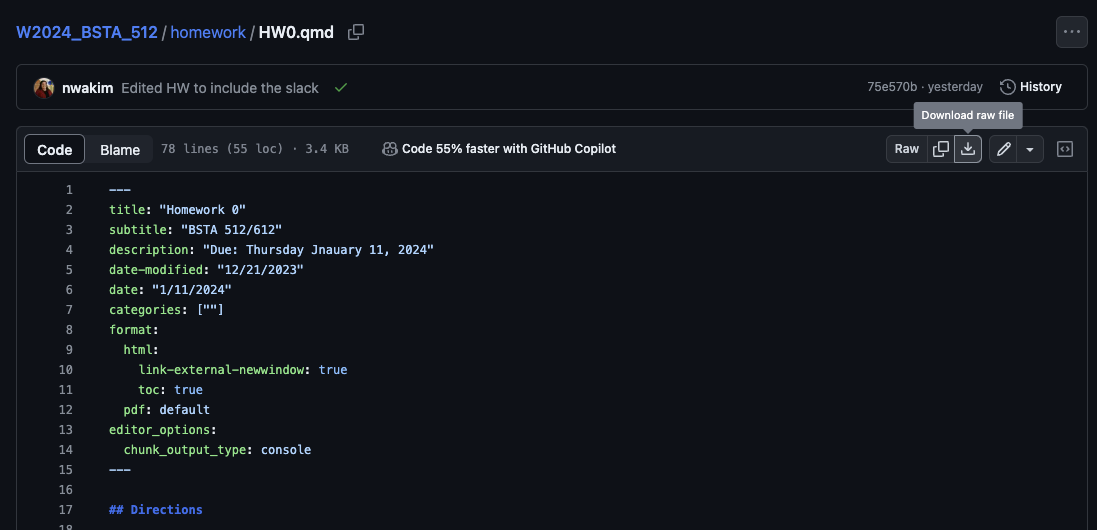
\includegraphics{HW0/HW0_github.png}
\item
  Click the ``Download raw file'' icon
  (
\includegraphics[width=0.26042in,height=\textheight]{HW0/download_icon.png})
  to download the \texttt{.qmd} file. This will likely download the file
  into your ``Downloads'' folder. It is up to you to move the file into
  the appropriate folder.
\item
  Please rename you homework as \texttt{Lastname\_Firstinitial\_HW0.qmd}
  . This will help organize the homeworks when the TAs grade them.
\item
  Please also add the following line under
  \texttt{subtitle:\ "BSTA\ 512/612"}:
  \texttt{author:\ First-name\ Last-name} with your first and last name
  so it is attached to the viewable document.
\item
  Edit the document with your explanations and code. If you are writing
  out an answer or calculating by hand, you can take a picture of your
  work and embed it within the \texttt{.qmd} file. The pictures will be
  viewable on the \texttt{.html} file.
\item
  Please upload your homework to this Sakai assignment. \textbf{Upload
  both your \texttt{.qmd} code file and the rendered \texttt{.html}
  file}.
\end{enumerate}

These instructions will not appear on every homework. You may come back
to this page for reference.

\hypertarget{purpose}{%
\subsubsection{Purpose}\label{purpose}}

This homework is meant to introduce yourself to me and your peers. In
the first class, we will all briefly introduce ourselves, but we don't
have enough time in-depth introductions. Thus, I'd like you to share
some information with the class over Slack.

\hypertarget{grading}{%
\subsubsection{Grading}\label{grading}}

Grading will be done as a check/no check for turning in your work. If
you are stressed about time, please turn in whatever you have completed.

\hypertarget{questions}{%
\subsection{Questions}\label{questions}}

\hypertarget{question-1}{%
\subsubsection{Question 1}\label{question-1}}

Please upload a picture of yourself
\href{https://join.slack.com/t/bsta512613w2024/shared_invite/zt-29g7biioz-XhPs~tj8xwL1GajEw9YlTg}{to
Slack}. Please follow the below steps to add a picture of yourself in
Slack:

\begin{enumerate}
\def\labelenumi{\arabic{enumi}.}
\tightlist
\item
  Go to the top right corner in Slack and click your profile picture.
\item
  Click ``Profile.''
\item
  In the picture of the clip art person, click ``Upload Photo'' in top
  right corner.
\item
  Upload a picture file of yourself.
\end{enumerate}

\emph{Please include the picture you used below. This will make sure we
are all able to insert a picture within Quarto. It will also make sure I
can see the photo within the \texttt{.html} file.}

\hypertarget{question-2}{%
\subsubsection{Question 2}\label{question-2}}

Provide a pronunciation of your name: Please follow the below steps to
add an audio and written pronunciation of your name in Slack:

\begin{enumerate}
\def\labelenumi{\arabic{enumi}.}
\tightlist
\item
  Go to the top right corner in Slack and click your profile picture.
\item
  Click ``Profile.''
\item
  To the right of your name, click ``Edit.''
\item
  Under ``Name Recording,'' click ``Record Audio Clip.''
\item
  Please say your name once at a normal pace then once slowly. Please
  listen to my audio for an example.
\item
  You may also edit the written pronunciation of your name. This is
  optional. I realize that doing this is may require a lot of time
  researching phonetics.
\end{enumerate}

\hypertarget{question-3}{%
\subsubsection{Question 3}\label{question-3}}

Please complete the \href{https://whenisgood.net/53kgg2b}{following
whenisgood poll} so that we can schedule office hours. Please use a
unique identifier (does not have to be your name), so that I can make
sure each student can attend at least one office hour.

\hypertarget{question-4}{%
\subsubsection{Question 4}\label{question-4}}

Completion of this question is optional. If you are comfortable sharing
your pronouns, please edit your name in Slack to include them. For
example, I have changed my name to be ``Nicky Wakim (she/her)''. If you
prefer to not share your pronouns, then I will refer to you using
they/them pronouns.

\hypertarget{question-5}{%
\subsubsection{Question 5}\label{question-5}}

Please post an introduction in the \texttt{\#random} channel on Slack.
You \textbf{\emph{do not need}} to include all of the below items, but
your introduction \textbf{\emph{may}} include information like:

\begin{itemize}
\tightlist
\item
  Preferred name
\item
  Pronouns
\item
  Are you new to Portland?
\item
  Career interests
\item
  Hobbies
\item
  Family, children, and/or fur babies
\item
  Favorite/recent adventures, restaurants, TV shows, books, podcasts,
  games, etc.
\item
  Willingness to join a study group
\item
  Motivation for taking the course
\item
  Anticipated Winter trip/activity
\item
  Any resolutions/vibes/outlooks that you are thinking about as we start
  the new calendar year/quarter
\end{itemize}

Please feel free to get creative with what you share! You don't need to
adhere to this list.

\hypertarget{question-6}{%
\subsubsection{Question 6}\label{question-6}}

Completion of this question is only necessary if you have
accommodations. If you have any learning accommodations, please email me
about your needs. I should receive a direct email from the Office of
Student Access, but it is important that we discuss how accommodations
will translate to our class.



\end{document}
